        \documentclass{standalone}
        \usepackage{tikz}
        \begin{document}
        \fontsize{16px}{16px}\selectfont
        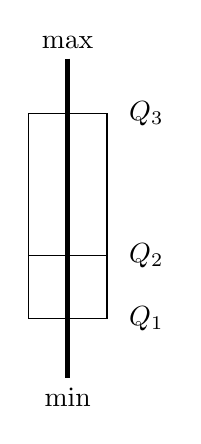
\begin{tikzpicture}

    \draw (0,0) -- (1,0) -- (1,0.8) -- (0,0.8) -- (0,0);
    \draw (0,0.8) -- (1,0.8) -- (1,2.6) -- (0,2.6) -- (0,0.8);
    \node at (0.5,3.5) (nodeA) {max};
    \node at (0.5,-1) (nodeB) {min};
    \node at (1.5,0) (nodeC) {$Q_1$};
    \node at (1.5,0.8) (nodeD) {$Q_2$};
    \node at (1.5,2.6) (nodeE) {$Q_3$};
    \draw[ultra thick](nodeA) -- (nodeB);
        \end{tikzpicture}
        \end{document}
